\section{ART Model}
\label{sec:model}

\begin{figure}[htbp]
	\hspace{0ex}
	\vspace{0ex}
	\centering
	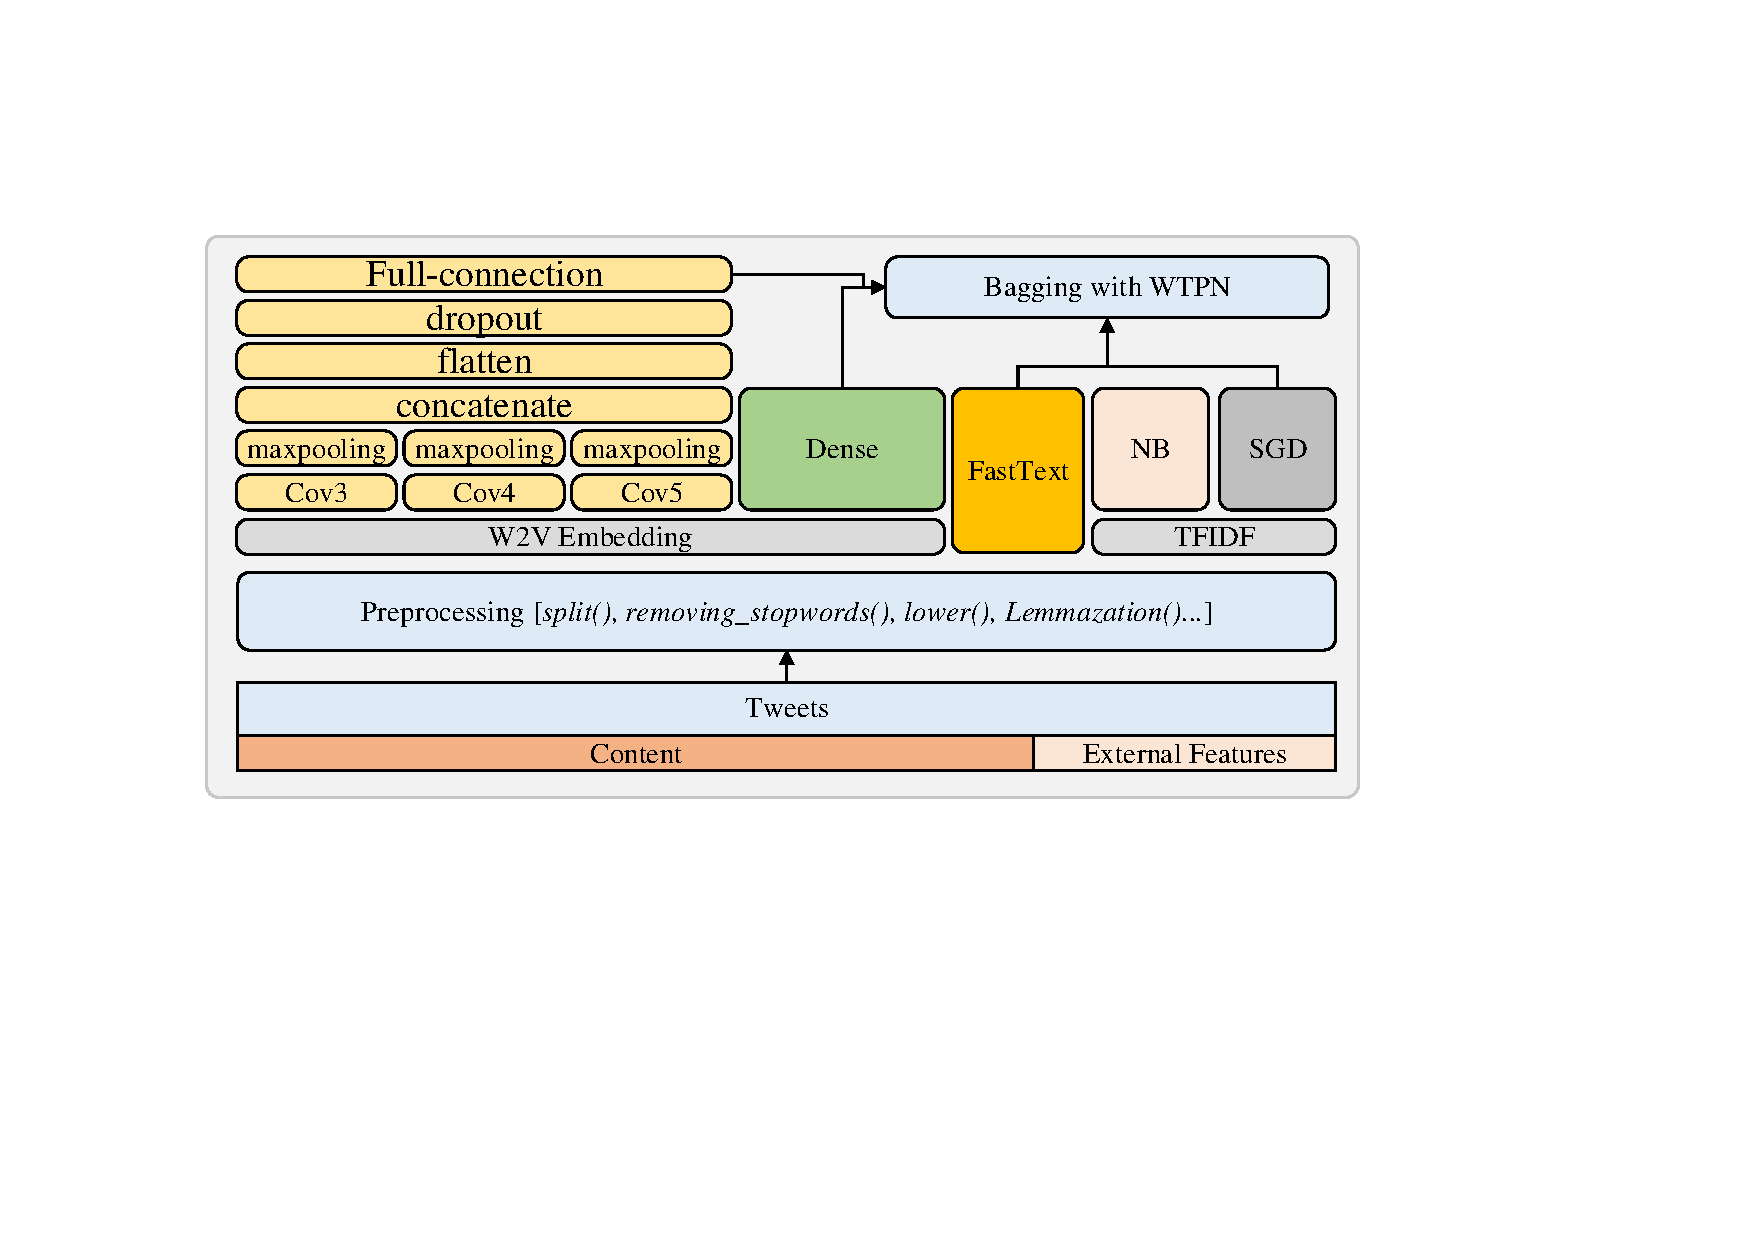
\includegraphics[width = \textwidth]{fig/structure}
	\caption{Architecture of ART}
	\label{fig:architecture}
\end{figure}

Aggregated model \cite{DBLP:conf/iccl2/Soto-FerrariCEH19, DBLP:conf/icccsec/WenYTWZSTYW18, DBLP:conf/wsc/LaippleMSWF18} aggregates different basic models as its components. With a proper aggregation strategy, the aggregated performance is usually better than that of the basic model. It is well established that the multiple components balance each other to reduce overfitting. Also, the most suitable classifier for different types of features is changing, and therefore multiple components are more likely to contain the proper classifier. Consequently, we using the aggregated model in ART to promote the performance of rumor tracking. 

\subsection{Architecture}
\label{sec:architecture}
The architecture of ART is shown in Fig. \ref{fig:architecture} . As it shows, the input of  ART consists of two types of features, which includes content features and social features. Then, all features are embedded and sent to basic components.  Some components such as TextCNN and Dense use word-to-vector embeddings and the other components use own embedding methods. Next, each trained component makes its prediction separately. Finally, we add the predictable results of all components and generate a final prediction by a voting based aggregation algorithm.

\subsection{Preprocessing and Embedding}
\label{sec:process_embedding}
The textual content is one of the most important features in the rumor tracking task. The length of the textual content is short, which is restricted within 140 words. Usually, the spelling in tweets is causal with symbols mixed in it. Consequently, we clean the content before inputting them into the model. The prepossessing in NLP is roughly immobilized, we only  make some minor adjustments. In this work, we adopt splitting on tweets, then removing the punctuation and special characters. Next, we turn all characters into lowercase. Finally, we adopt lemmatization on all words.

We find that the embedding strategies have a significant impact on the performance of ART. Therefore, we try different embedding strategies to find the most proper one. There are three commonly used embedding strategies: pre-trained embedding, self-trained embedding, and random embedding. Pre-trained embedding is trained on large-scaled corpus, and the most representative ones are GloVe \cite{DBLP:conf/emnlp/PenningtonSM14} and Google News embedding \cite{googlenews}. The self-train embedding is to train embedding on the current dataset. And the random embedding is to assign each word with a unique embedding randomly. In this work, we try all three embedding strategies and the detailed performance is introduced in Section \ref{sec:experiment}. By comparing them, we finally choose random embedding as the embedding strategy in ART.

\begin{algorithm}[tbp]
	\caption{Voting based ART}
	\label{algorithm:art}
	\LinesNumbered % show line numbers
	\KwIn{$K_y = \left\{y_F', y_T', y_B', y_N', y_S' \right\}$: outputs of all components;}
	\KwOut{$R$: predictable result of ART;}
	\textbf{Initialize:} Outputs of ART: $y' = [0]*m$, $R = 0$ \;
	
	\For{$y_i'$ in $K_y$}{
		$r = 0$\;
		$r = argmax(y_i')$\;
		$y'[r] ++$;
	}
	
	$R = argmax(y')$
\end{algorithm}

\subsection{Procedure of ART}
As shown in Fig.~\ref{fig:architecture}, after embedding, we send \textbf{content features} into TextCNN, SGD, and FastText. These three components are trained respectively until getting convergence. When predicting, each component outputs an m-dimensional vector $y'$ after the softmax layer. Each component in $y'$ suggests the probability that the content belongs to this category. Despite some content features, the tweets contain plenty of \textbf{social features}. As introduced in Section \ref{sec:problem}, the tweet's branch or thread unknown in advance. Consequently, we omit some features that contain external information about the branch or thread. Finally, we choose "screen name" and "hashtag" as the social features in ART. We treat the social features as words and add them to the tweets. Then we send the tweets with social features added into NB and SGD. 

With all components in ART trained, we aggregate them and give the final prediction on the rumor tracking task. Generally, there are two commonly used aggregation methods: \textbf{joint training} and \textbf{respective training}. Joint training means all models have one shared loss function, and all parameters are updated together. When predicting, the aggregated model directly outputs the final prediction. Respective training means we train each component respectively. When predicting, each component makes its prediction result. In ART, all results are aggregated by a voting strategy. It means that each component votes to a category and the category with the most votes is the final prediction result and the results are combined via an algorithm. The aggregation details of ART is shown in Algorithm~\ref{algorithm:art}. We denote the predictable result of a component as $r$ and the predictable result of ART as $R$. The inputs of Algorithm~\ref{algorithm:art} is the outputs of all components, which is denoted as $K_y = \left\{y_F', y_T', y_B', y_N', y_S' \right\}$. Each element in $K_y$ is an m-dimensional vector, and we get the predictable result of it firstly (Line 4). Then we treat each predictable result of components as a vote and record the counts on each category (Line 5). Finally, the category with the most votes is the predictable result of ART (Line 7). 
